\chapter{RePlay: Contextually Presenting Learning Videos Across Software Applications}
Complex activities often require people to work across multiple software applications. However, people frequently lack valuable knowledge about at least one application, especially as software changes and new software emerges. Existing help systems either lack contextual knowledge or are tightly-knit into a single application. We introduce an application-independent approach for contextually presenting video learning resources and demonstrate it through the RePlay system. RePlay uses accessibility \textsc{api}s to gather context about the user's activity. It leverages an existing search engine to present relevant videos and highlights key segments within them using video captions. We report on a week-long field study ($n\!=\!7$) and a lab study ($n\!=\!24$) showing that contextual assistance helps people spend less time away from their task than web video search and replaces current video navigation strategies. Our findings highlight challenges with representing and using context across applications.

\begin{figure}[t!]
%\vspace{-0.2in}
\centering
  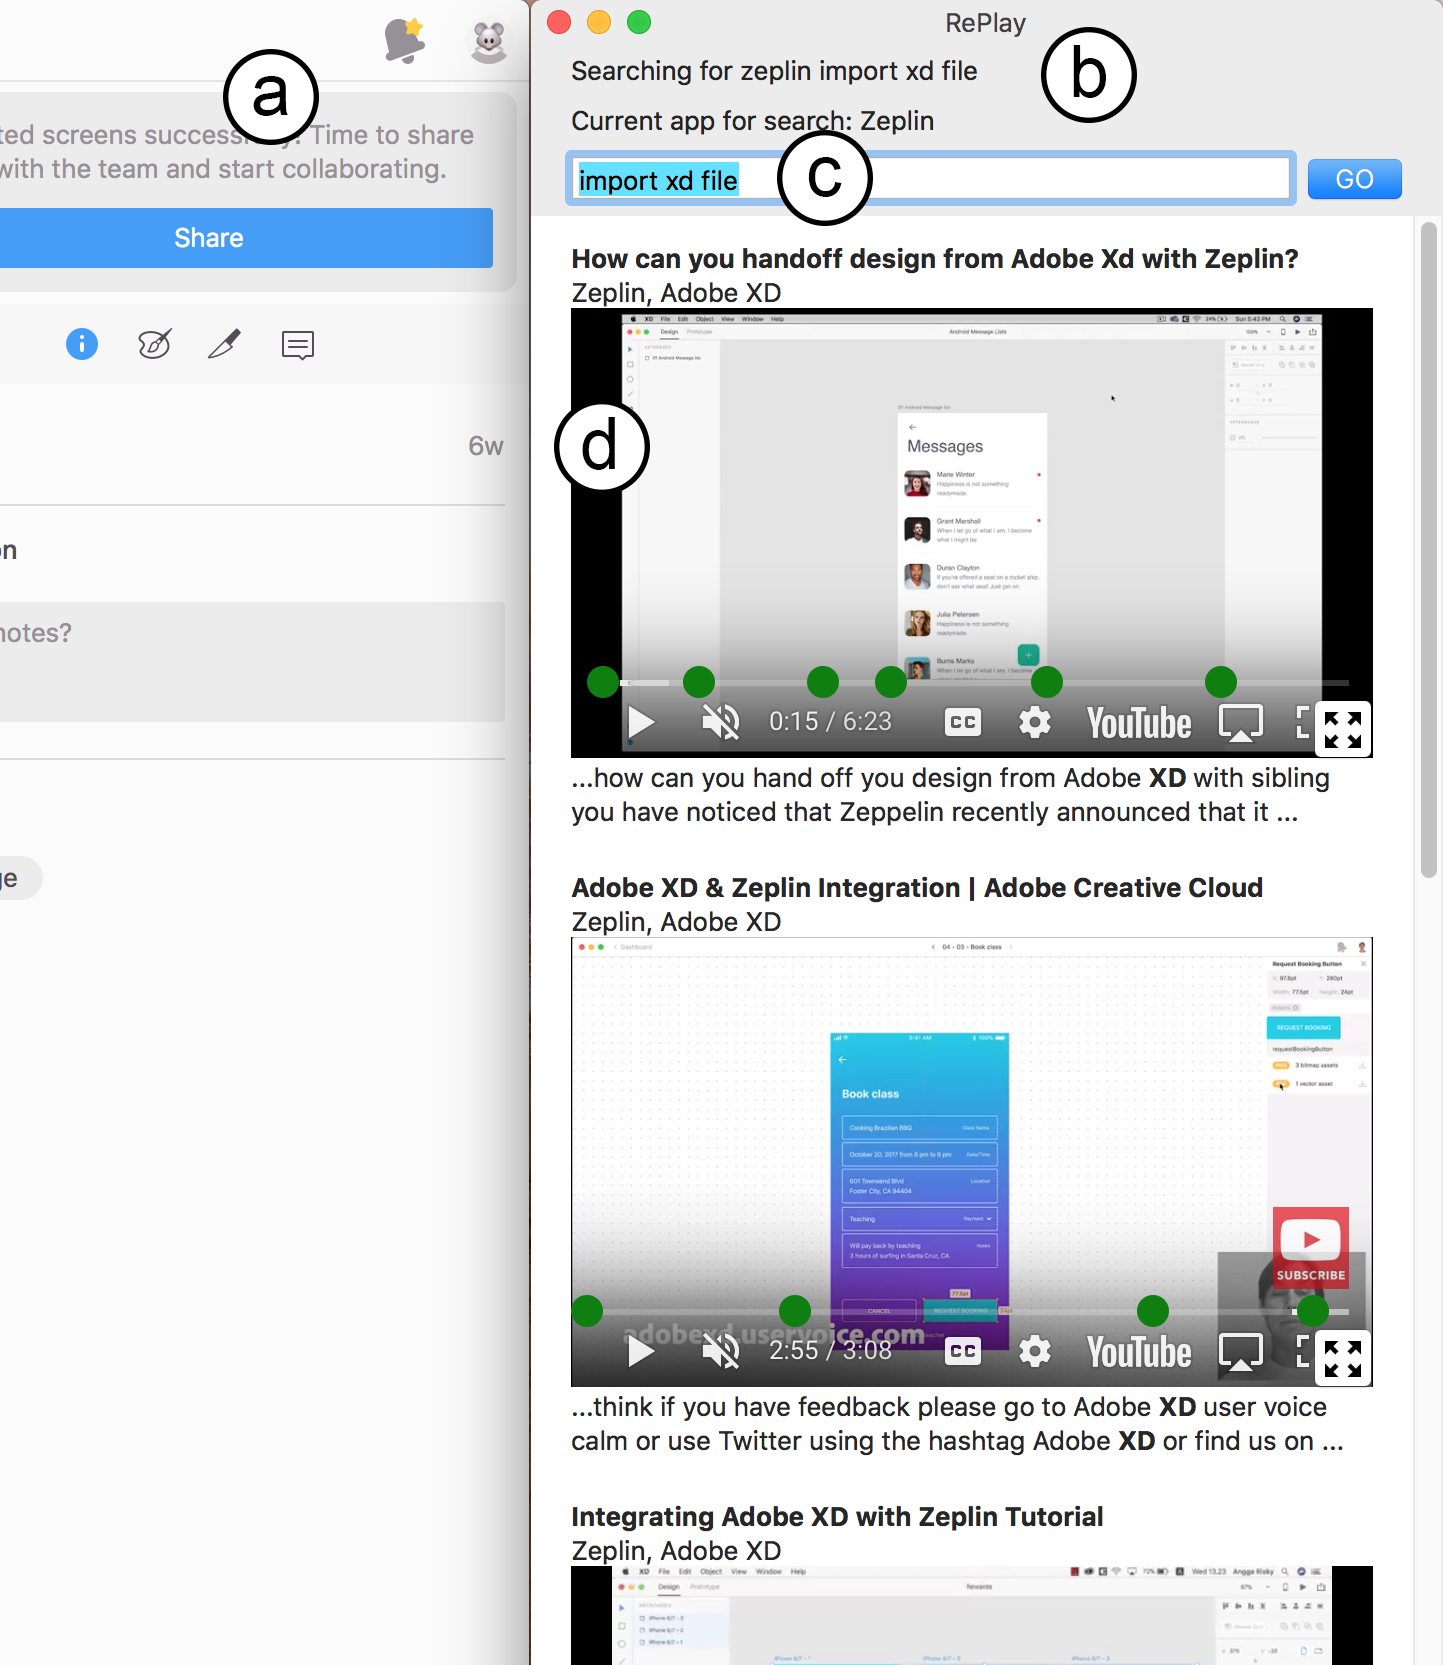
\includegraphics[width=1\textwidth]{replay/figures/replay-interface.png}
  \caption{RePlay - shown to the right of Zeplin (a) - includes a status area (b) and search field (c) at the top. Video results (d) include timeline markers and caption excerpts to highlight moments relevant to the user's query and context.}
  \label{fig:replay-interface}
%   \Description[A screenshot of RePlay's interface next to the application Zeplin.]{A screenshot of RePlay's interface next to the application Zeplin. RePlay comprises a status area, a search field, and video results. Timeline markers and caption excerpts overlaid on video results highlight moments relevant to the user's query and context.}
  \vspace{-0.20in}
\end{figure}

\section{Introduction}
Most software activities span multiple applications. The slogan ``there's an app for that'' illustrates that we live in a world filled with specialized apps that each focus on a few specific tasks. To accomplish larger activities requires composing multiple applications together into a ``toolbelt'' \cite{Sumner1997}. For example, designing an interface might comprise drawing a logo in Illustrator, mocking up a prototype in Sketch, adding animations using Flinto, and presenting it to a client using Keynote. Analyzing data might involve formatting it using Python, viewing and graphing it in Excel, modifying graph aesthetics in Photoshop, and reporting results in Word. Toolbelts help users tailor custom ecosystems and support distributed innovation. However, this bricolage creates a user experience problem: even with design guidelines, every application is different \cite{Beaudouin-Lafon2018}. As new applications appear and existing ones change, few people are fluent experts in all the steps towards their goals.

Presenting learning resources in-application \cite{Grossman2010a, Chilana2012, Matejka2011a, Matejka2011, Brandt2010, Ichinco2017} and augmenting search queries with contextual information \cite{Ekstrand2011, Brandt2010} can offer a more fluid experience with lower cognitive load. However, existing solutions require deep integration with applications. And since today's applications are ``walled gardens''  with limited integration across software vendors \cite{Beaudouin-Lafon2018}, help resources typically focus on one application at a time. This leaves gaps when users want to move from one application to another (\textit{e.g.,} export an Adobe \textsc{xd} prototype to Zeplin) or interleave applications (\textit{e.g.,} coding a website in Sublime while debugging in Chrome and resizing graphics in \textsc{gimp}). 

% Web search results can of course include community-created resources that span applications. However, generic web search poses two problems. First, search is blind to relevant contextual information that could connect users to better resources \cite{Ekstrand2011, Kraft2005, Finkelstein2002}. Search engines place the burden on users to articulate an appropriate query, an almost paradoxical requirement for users who are there because they don't know the domain \cite{Russell2011}.  Second, search is divorced from the application UX, requiring users to bounce back and forth to connect the content \cite{Fourney2014Intertwine}. These challenges are amplified when users work with multiple applications, each with its own terminology and conventions.

We introduce an application-independent approach for contextually presenting video learning resources. We embody this approach in the RePlay system (\autoref{fig:replay-interface}), which enables users to search for learning videos based on their application usage. RePlay gathers application context using system accessibility \textsc{api}s. It extends online video search and cues videos to relevant segments based on their captions. We focus on video assistance because despite video's growing popularity (Cisco predicts that by 2021, 82\% of all internet traffic will be video \cite{Cisco}), searching and browsing videos remain cumbersome \cite{Kim2014, Pavel2014, Pavel2015}. Video is popular for content creators as it is often easier to author than tutorials or diagrams (which require careful curation). Learners value video for its efficacy in communicating complex or continuous visual actions such as brushing or setting parameters \cite{Chi2012}. However, interacting with videos remains difficult because they are harder to navigate and scan for steps than text \cite{Chi2012}.

%for its popularity as a learning resource \cite{Chi2012, Pongnumkul2011, Nguyen2015}, especially for visual tasks
%its simultaneously the most useful thing for many tasks and also the least well supported by current search interfaces
% while video has become increasingly ubiquitous and easy to create -- ... -- searching and browsing remain cumbersome.

We report on two studies observing how people use RePlay and web video help: a week-long field study ($n\!=\!7$) and a lab study ($n\!=\!24$) where half the participants used RePlay and half used web video search. Both studies used visual design as the domain, as video is especially helpful for visual tasks \cite{Pongnumkul2011}. The field study examined how designers with varying experience used RePlay in-situ. Participants used an average of 17 different applications in a week, emphasizing the importance of system-wide integration. Our findings also suggested that contextual video assistance benefits targeted tasks more than open-ended ones. The lab study found that contextual video assistance helps people spend less time away from their task than web video search, and replaces strategies typically used in navigating between and within videos. This work makes the following contributions:

\begin{enumerate}
    \item An application-independent method for finding relevant clips in learning videos that leverages user context,
    \item the RePlay system, which demonstrates this method using accessibility \textsc{api}s and online video corpora, and
    \item insights from two studies that highlight the importance of multi-application support and the promise of cross-application search.
\end{enumerate}




% replay is an example implementation of such a tool / embodiment of this approach / design probe to illustrate how this could be done, and investigate whether it helps people. / show that this is a viable direction for future research 

% people dream of this thing. we offer a new path to achieve aspects of that goal. knitting help together lowers the friction between applications

% arg 1: lack of integration creates friction that our work mitigates
% ****arg 2: if you need to assemble a buncha tools that all work differnetly you won't know them all
% arg 3: the seams / hand off points require guidance

%Currently, it is difficult for users to get effective guidance when tasks span applications: in-situ help and official documentation is only available at the individual application level, and community-created resources that sometimes do span applications move the user out of their workflow and into the browser. 


%include Google YT timeline marker result as an example
%have IoT example for camera-ready video
% somewhere also mention accessibility for all argument

%watching ppl use 2 different video interfaces taught us what a good video interface should be (wouldn't be able to find this otherwise)

\section{Related Work}
%YouTube also contains many videos that specifically address cross-app workflows (e.g., exporting content from one application and importing it into another). 
This work builds on prior contextual search and video segmentation work with a novel focus on multi-app activities.
%This necessitates an application-general approach for detecting context and a domain-general approach for searching and ranking. 

\subsection{Multi-app activities are hard to support consistently}
People often work across multiple applications that each support an individual task to perform higher-level activities \cite{Sumner1997}. Help systems for such applications tend to focus on their individual tasks rather than the transitions and interactions between them \cite{Norman2005}. Implementing system-wide assistance that captures activity context is difficult, as every application has its own conventions and interface, and software interoperability tends to be limited \cite{Beaudouin-Lafon2018}. Accessibility \textsc{api}s are one useful entry point for diverse system-wide extensibility, including visualizing user behavior \cite{Matejka2013}, voice control \cite{Li2017, Zhong2014}, and modifying or enhancing existing user interfaces \cite{Dixon2014, Stuerzlinger2006, Chang2011}.
RePlay uses accessibility \textsc{api}s for detecting system-wide application context.
% one inspiration for this work is the emergence of creative professionals live streaming their work. these live streams offer a more holistic view than ``help'' because viewers can see how specific functions fit together. 

\subsection{Application context improves relevance and presentation of learning content}
The most teachable moment for software tasks is often when the user is actively working... but stuck. In-task help for a specific goal is one of the biggest reasons people seek web \cite{Lafreniere2013a} and video \cite{AlamAnik2015} tutorials. However, tutorials tend to show a full task from start to finish, much of which may not be relevant to the user's current goal. This leaves it to the user to both find a relevant tutorial and locate the segment(s) within it that contains the needed information.

Effectively searching the Web is an acquired skill; coming up with the right keywords and search settings can be difficult, especially for novices \cite{Russell2011}. In addition, web search environments lack context that human tutors use to proactively offer help and tailor feedback \cite{Schon1983}. Adding contextual terms automatically to search queries (\textit{e.g.,} \textsc{os} version, application, recently-used tools) can help improve the relevance and utility of search results without requiring the user to know app-specific terminology \cite{Ekstrand2011, Brandt2010, Matejka2011a}. RePlay augments queries with the current application name and uses context from both the current and recently-used applications to support cross-app activities when ranking search results.

Adding contextual cues to search results provides information scent that can help users more quickly and easily navigate the results (\autoref{fig:replay-green_markers}). Such cues show how and why a result is relevant to the user's own situation and direct them to the relevant information within a result \cite{Ekstrand2011, Fourney2014Intertwine}. RePlay expands these ideas to video, displaying contextual cues for recently-used applications and tools.

Bringing learning resources directly into applications reduces the need for context switching. For example, proactively recommending content in-situ based on user context can lead users to resources they might not have even thought to search for \cite{Matejka2009, Fraser2016, Chilana2012, Matejka2011, Ichinco2017}. In-app search also helps users stay focused on their task while learning \cite{Lafreniere2014a, Fraser2016, Chilana2012}. RePlay brings these strategies into an application-independent system, functioning alongside the user's applications.

\subsection{Videos are helpful for learning but hard to navigate}
Videos are popular for many kinds of tasks, especially visual ones, because they show clear demonstrations that might be harder to explain or understand in text \cite{Chi2012, Pongnumkul2011}. Videos are widely available and relatively easy to make. Software is always being updated, and new video demonstrations are constantly added to popular platforms by the user community to keep up with updates and current trends. However, while text-based documents are easy to skim and search, videos are not \cite{Pavel2014, Pavel2015, Kim2014}. The predominant video search approach displays results as thumbnail images with a title and summary (\textit{e.g.,} YouTube, Vimeo). This presentation only provides a broad overview without cues about matching content; prior work has shown that people look for indications of how search results are relevant to their query \cite{Hearst2009Book}. Navigating within videos is typically limited to hovering across the timeline with a small visual preview.

Automatically dividing videos into conceptual chunks can improve peoples' ability to find useful information for their task \cite{Pongnumkul2011, Chi2012, Banovic2012, Nguyen2015, Grossman2010a, Matejka2011}. RePlay uses captions to select relevant clips \cite{Pavel2014, Pavel2015, Girgensohn2005}. Automatic clip selection plays a limited but growing role in web search. Google displays a ``suggested video clip'' \cite{Sullivan2018} as the automated summary for some searches, and Bing's ``smart motion preview'' feature \cite{Bing} shows a 30-second preview for video search results. In contrast, RePlay focuses on searching with and presenting results within application context. Chi et al. \cite{Chi2012} showed people benefit most from a mix of text and video; RePlay combines video and text instruction by presenting captions with videos for both navigational and learning assistance.

Methods for navigating between video segments include interactive timeline markers \cite{Matejka2011, Grossman2010, Kim2014, Banovic2012, Kim2014a}, thumbnail images \cite{Kim2014a, Pongnumkul2011, Banovic2012, Grossman2010a, Chi2012, Pavel2014}, transcript text \cite{Kim2014a}, and clickable elements overlaid on the video \cite{Nguyen2015}. Like Ambient Help \cite{Matejka2011}, ToolScape \cite{Kim2014}, and Chronicle \cite{Grossman2010}, RePlay overlays markers on the timeline indicating command or tool use. We use timeline markers over other options as they take up little space and allow for pop-up text previews, which aid browsing. While prior work marks \textit{all} instances of tool use or interface actions, RePlay marks only \textit{contextually-relevant} moments (recently-used tools and words from the user's query) to reduce clutter and unnecessary detail in a small interface.


%As a result, the learning materials online differ for each application as well. Different keywords may be necessary to find help for a given task depending what application you are using for that task.
%But maybe we don't need application-specific knowledge. Maybe we can just make use of existing system-wide functionality, get the minimum information it provides for most applications, and use that to augment existing search engines just enough to support these activities a little better.

%This requires the user to translate their own context and situation back and forth with that in the browser. Users must determine what of their context might potentially be relevant and articulate a search query appropriately, determine which search results might be relevant to this context based on their information scent, and finally map the instructions received back to their own unique situation. (maybe move to a separate section?)
\section{RePlay System}
This section describes RePlay's user interface, context detection, and system architecture.
%RePlay is a desktop application that allows users to search for contextually-relevant video clips for any accessibility-enabled desktop application. It leverages large online video corpora, searching video caption text for relevant moments. The RePlay prototype investigates the efficacy and challenges of cross-app contextual search.

\begin{figure}[b!]
\centering
\vspace{-0.2in}
  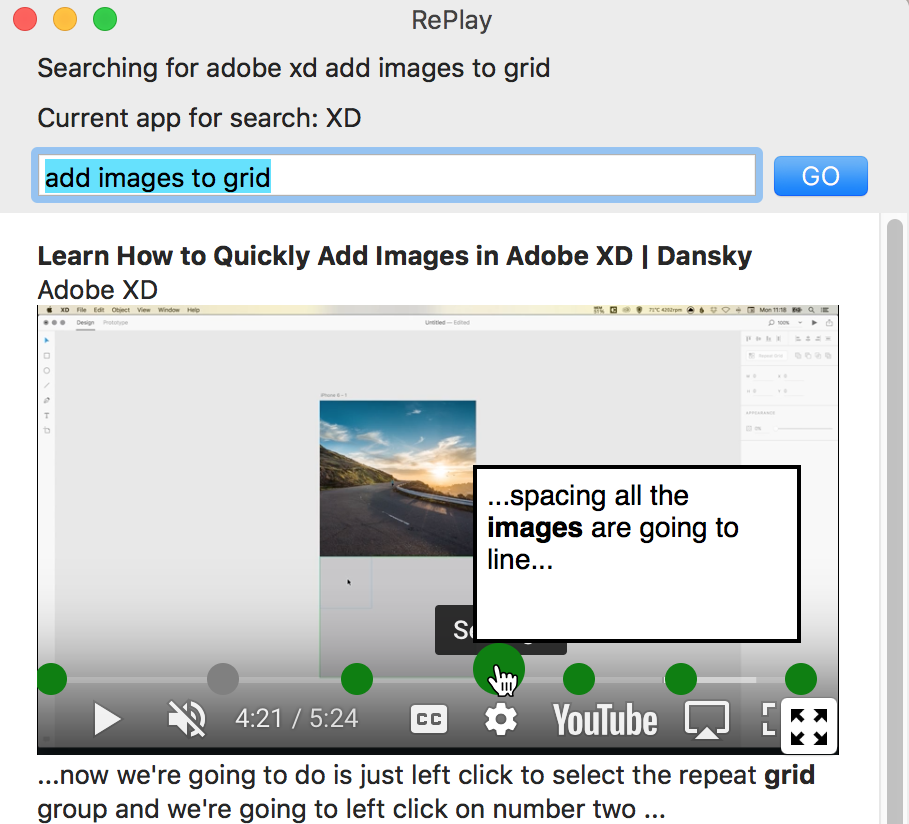
\includegraphics[width=\textwidth]{replay/figures/green_markers.png}
  \caption{RePlay overlays green markers on the video timeline to indicate moments where the captions match a user's search term. Mousing over a marker shows a pop-up with an excerpt from the captions at that moment; clicking it plays the video from that moment. }~\label{fig:replay-green_markers}
%   \Description[A screenshot showing green markers overlaid on a video result in RePlay.]{A screenshot showing green markers overlaid on a video result in RePlay. The user has searched for ``add images to grid'' in Adobe XD, and the top video result is titled ``Learn how to quickly add images in Adobe XD''. The video timeline has green dots on it, and the mouse is hovering over one. A pop-up shows a caption excerpt that says: ``...spacing all the images are going to line...'' with the word ``images'' bolded.}
  \vspace{-0.2in}
\end{figure}

\subsection{User interface}
The RePlay panel (\autoref{fig:replay-interface}) can be positioned and sized as desired; its default size is 465px \texttimes 1055px. It is designed to fit next to the user's primary applications to minimize switching windows. The narrow pane makes videos small but easier to browse and watch in context. The interface comprises a status area, search field, and video results.

The status area updates as the user works, displaying the name of the last tool clicked and the current application (\autoref{fig:replay-status}). ``Tools'' refer to interface elements or commands within an application. The status area provides awareness of what context RePlay will use for search (\textit{i.e.,} so the user does not need to include the application name in their search query). When the user initiates a search, the status area updates to show the query (\autoref{fig:replay-interface}b).

As the user works, the search field updates with the name of the last tool clicked (\autoref{fig:replay-status}). Users can edit or delete it to form their own query. Pressing the \textsc{go} button or return key triggers a search. RePlay displays the top five resulting videos, each cued to start at a relevant moment. A two-line excerpt from that moment's caption appears below the video with query words highlighted in bold \cite{Hearst2009}.

Often, videos have multiple moments that may be relevant. RePlay renders green markers on the video timeline to indicate these moments. Mousing over a marker invokes a pop-up text area displaying a caption excerpt with words from the query in bold (\autoref{fig:replay-green_markers}). This pop-up obscures YouTube's default thumbnail pop-up but provides more useful information, as software videos tend to show an entire screen and shrinking this to a thumbnail makes it hard to see. Clicking a marker starts the video from that moment. 

\begin{figure}[b!]
\centering
\vspace{-0.2in}
  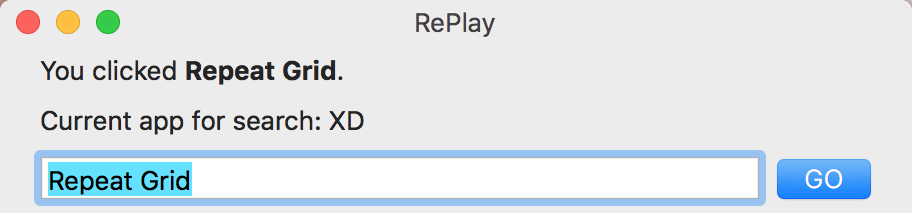
\includegraphics[width=\textwidth]{replay/figures/replay_status.png}
  \caption{RePlay's status area displays tool names after they are clicked and adds them to the search field. }~\label{fig:replay-status}
%   \Description[A screenshot of RePlay's status area.]{A screenshot of RePlay's status area. It reads, ``you clicked Repeat Grid'', and has the tool name ``Repeat Grid'' included in the search field.}
  \vspace{-0.2in}
\end{figure}


RePlay also displays contextual cues \cite{Ekstrand2011} on search results (\autoref{fig:replay-context_cues}). For each video, RePlay lists the three most-recently used applications that are mentioned in the video (\autoref{fig:replay-context_cues}a). This list is especially useful when users move between applications and want videos that mention both the current and recent applications. RePlay renders grey timeline markers to indicate moments where recently used tools are mentioned (\autoref{fig:replay-context_cues}b). Caption pop-ups italicize tool names.


\begin{figure}[b!]
\centering
\vspace{-0.2in}
  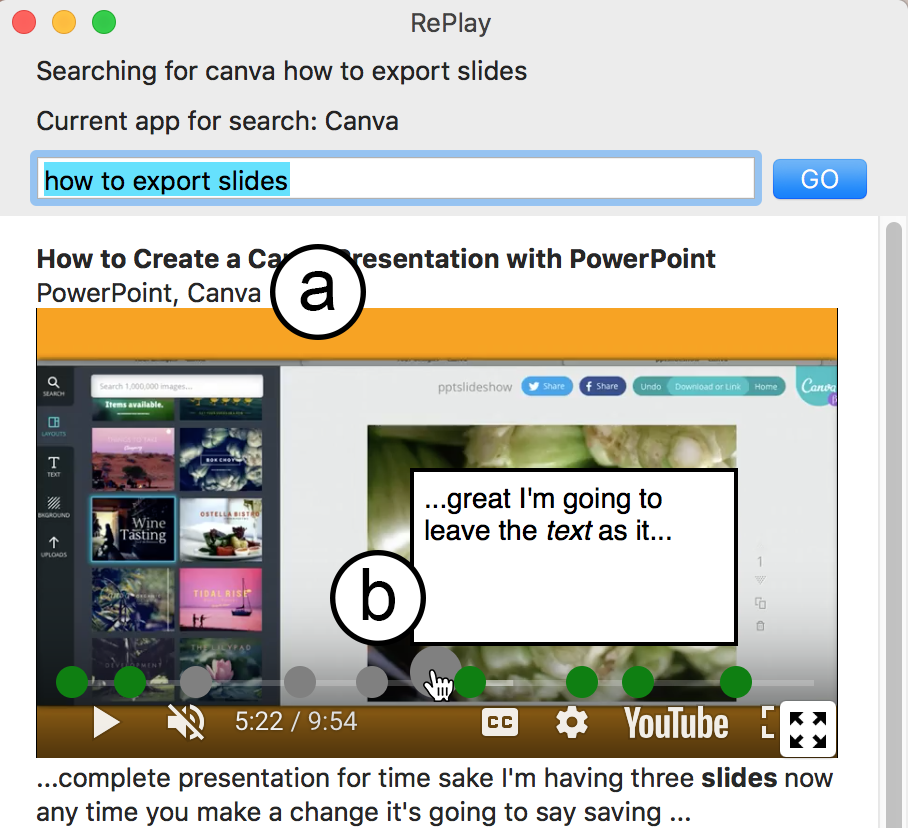
\includegraphics[width=\textwidth]{replay/figures/context_cues.png}
  \caption{RePlay displays contextual cues based on recent app and tool use. a) RePlay lists the three most recent apps that the video mentions. b) Grey markers indicate mentions of recently-used tools. In this example, the user recently used the ``text'' tool in Canva. Mousing over a marker shows a caption excerpt; clicking a marker plays the video. }~\label{fig:replay-context_cues}
%   \Description[A screenshot showing grey markers overlaid on a video result in RePlay.]{A screenshot showing grey markers overlaid on a video result in RePlay. The user has searched for ``how to export slides'' in Canva, and the top video result is titled ``How to create a canva presentation with PowerPoint''. The video timeline has grey dots on it, and the mouse is hovering over one. A pop-up shows a caption excerpt that says: ``...great I'm going to leave the text as it...'' with the word ``text'' italicized.}
  \vspace{-0.2in}
\end{figure}

RePlay's panel shows all results at the same time, allowing users to quickly skim multiple videos, and browse other results while one video plays. This ability to ``see inside'' multiple resources from a single page increases foraging efficiency \cite{Vermette2017, Glassman2016, Pavel2013}. 

Clicking the full-screen button in a video's bottom-right corner opens the video in a separate window that stays above all other windows while it is open, so that users can watch a video at a larger size when desired.

When the user switches to a new application and clicks a tool, RePlay automatically searches for the application name. This seeds the panel with app-relevant videos that give users a starting point.

\subsection{Detecting application context}
RePlay uses contextual information to augment a user's query and search within video results. The motivation for context-augmented search is to increase relevance, especially when users don't know what to ask for. However, if not done well, adding terms has the opposite effect: excluding relevant results and/or presenting irrelevant ones \cite{Finkelstein2002}. We tried several heuristics with RePlay; the current implementation includes the three most recent applications and tools.

\subsubsection{How to detect context?}
RePlay leverages \textsc{os} accessibility \textsc{api}s to detect every click. On each click event, RePlay retrieves the name of the click's source application, the type of element clicked, and the element's accessibility description (when present). If the element is a button, checkbox, text field, slider, or menu item, RePlay stores it as a recent tool and updates the status area and search field with the tool's name. If the user switched applications since their last click, RePlay updates its status area to reflect the new application, and resets its list of recent tools.

\subsubsection{Challenges with detecting context via accessibility}
Extracting accessibility text obviates the need for hard-coded knowledge about specific applications. The challenge of this system-wide approach is that despite platform accessibility guidelines, applications vary widely in what accessibility they offer and how \cite{Hurst2010}.

In Mac\-OS, RePlay can always extract the application name and menu items. Buttons and other interface elements have accessibility labels in many applications (\textit{e.g.,} Adobe \textsc{xd}, Microsoft Office, iMovie, Tableau, Sketch), but not in others (often long-existing software, \textit{e.g.,} Photoshop). Applications differ in which accessibility fields they support and what information is in what field. For example, tool names may be in the \textit{Title}, \textit{Help}, \textit{Description}, or \textit{Value} attribute. RePlay checks all four, preferring them in that order. RePlay also gathers accessibility information for websites, as long as browser accessibility access is enabled. It is by default in Safari, and as an option in Chrome. Many sites implement accessibility labels (\textit{e.g., } Canva, Wordpress, Sketchpad, Snappa, G Suite). Those that do not still include some information by default (\textit{e.g.}, text area contents via the \textit{Value} attribute). RePlay infers website names from the \textsc{url} and website title.

\subsection{Video search \& ranking}
RePlay leverages existing online video search engines to retrieve video results. It then finds and ranks relevant clips within these videos (\autoref{fig:replay-system}). RePlay's architecture requires no prior understanding of the applications or videos; it relies on captions for clip extraction and ranking. Video authors often talk about things they are doing and provide tips about tools; captions thus provide narrative information beyond the visual content in the video that can be useful for learners.

\begin{figure}[b!]
\centering
\vspace{-0.2in}
  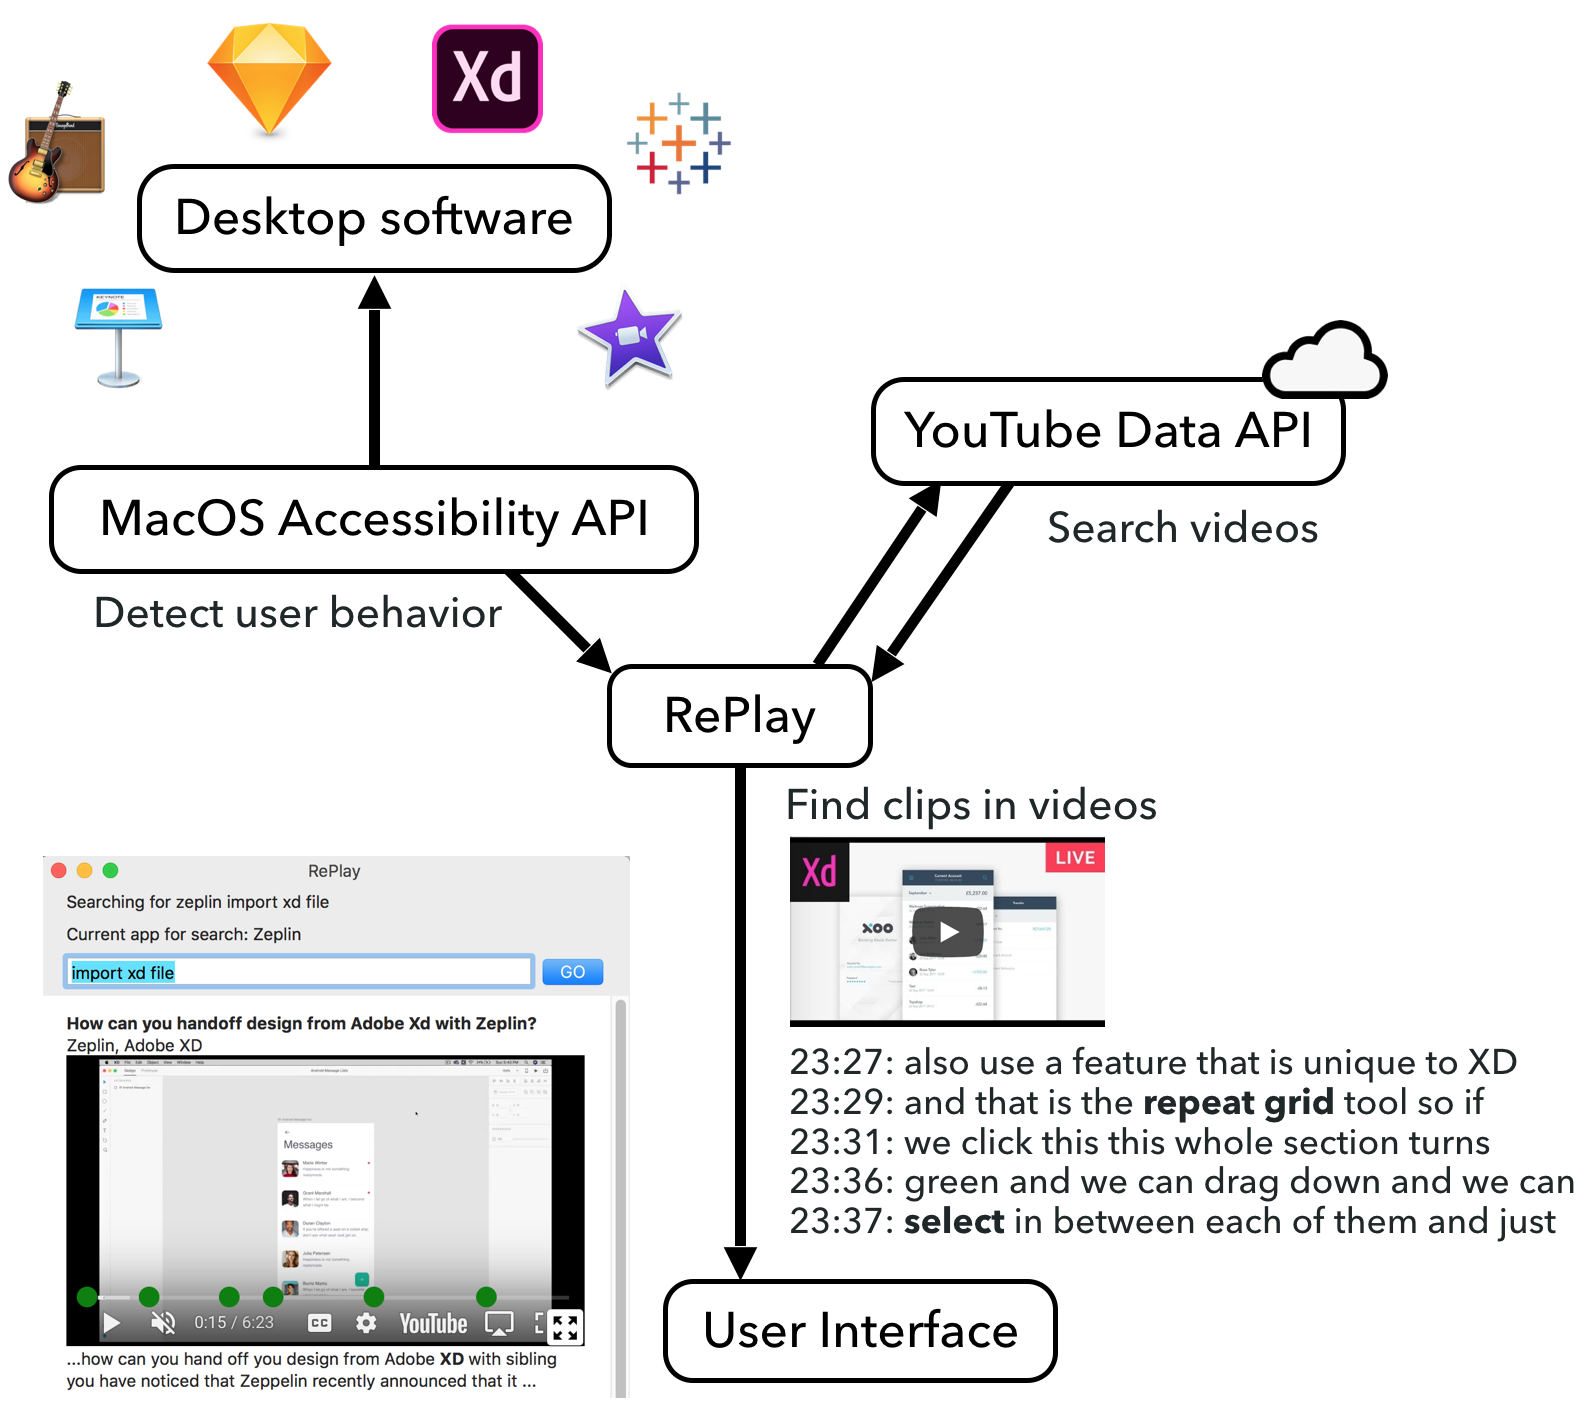
\includegraphics[width=\textwidth]{replay/figures/replay-system.png}
  \caption{RePlay uses accessibility \textsc{api}s to detect user context, which it uses to augment the user's query and to search and rank videos. RePlay finds matching clips by searching video captions for the user's query and recent tool names. }~\label{fig:replay-system}
%   \Description[A diagram showing the different components of RePlay and how they communicate.]{A diagram showing the different components of RePlay and how they communicate. The MacOS Accessibility API detects user behavior from desktop software and sends this to RePlay. RePlay searches videos using the YouTube Data API. RePlay finds clips in these videos and displays them in the user interface.}
  \vspace{-0.2in}
\end{figure}

\subsubsection{Available data}
RePlay's current video corpus comprises all English videos on YouTube that have a caption track. Most do: YouTube auto-generates captions by default. We used YouTube for its popularity and captions; any video search engine with an \textsc{api} could be used. For example, Vimeo (\url{vimeo.com}) and Dailymotion (\url{dailymotion.com}) also provide \textsc{api} access to videos and captions.

\subsubsection{Searching}
Video search requires more steps than document search, because captions are obtained separately. This two-step search means that issuing multiple queries with context terms added (such as tool usage) like prior work \cite{Ekstrand2011} would be too slow. To speed responses, RePlay constructs and issues a single query concatenating the current application's name with the user's query. Leaving context terms out of the query also ensures that the user-provided search terms are not ``washed out''. RePlay queries YouTube and selects its top five video results that have English captions and mention the current application in any of the title, description, or captions (to avoid results that may contain other keywords but do not pertain to the current application).

\subsubsection{Finding clips and re-ranking videos}
Several techniques automatically extract instructional video clips from screencasts of software use. The dominant approach leverages application usage \cite{Grossman2010, Lafreniere2014, Chi2012, Wang2018}, requiring that the video be recorded in an instrumented version of the software. Alternatively, computer vision can detect tool-selection events \cite{Pongnumkul2011, Matejka2011}, even without prior knowledge about the specific software \cite{Banovic2012}. To be application-independent and embed online videos directly without waiting to download and process them, RePlay instead uses metadata and caption text to rank and segment videos. 

For each video result, RePlay divides its captions into 30-second segments, searching each for the queried keywords (with stop words removed) and names of the three most-recently used tools in the current application. It ranks all segments by the total number of keyword matches. To break ties it uses number of tool name matches. The highest-ranked segment determines the video's start time. Timeline markers denote the top ten segments: green for those with a query term; grey if only a tool is mentioned. RePlay re-orders the video results based on the total number of matching clips. To break ties it uses the total number of matching keywords within the clips.

Although automatic captions are far from perfect, we found them to be sufficient for searching in RePlay. Captions are already an approximation of what the demonstrator is doing, so despite some errors, they work well enough for identifying potentially relevant moments. Having any aids for navigating within videos is still an improvement over standard viewers. Still, future systems could allow viewers to easily correct errors as they watch to improve caption accuracy for future viewers.

\subsection{Implementation}
RePlay is implemented as a Mac\-OS application in Swift. It uses the Mac\-OS Accessibility \textsc{api} to extract information from input events. For both studies, RePlay used a whitelist to only detect clicks in certain applications and websites. A blacklist could be used instead; we explore this in the discussion.

When a search is triggered, RePlay queries the YouTube Data \textsc{api}'s \texttt{search} method, which returns an ordered list of video \textsc{id}s. For each \textsc{id}, RePlay checks if English captions are available using YouTube's \texttt{get\_video\_info} method. If they are, this method's response includes a \textsc{url} that RePlay follows to obtain subtitles in \textsc{xml}, with time stamps for every 5 to 10 words. A search that returns all new videos can take up to a few minutes to finish depending on network speed, due to the multiple requests needed to retrieve captions for each video. To speed up future searches, RePlay caches all retrieved captions locally (since they are pure text, this takes up little space). This could be further improved by proactively caching results for common search queries and buffering results as they come in. RePlay's video player is implemented in Javascript on a custom server; it embeds a YouTube video in an \texttt{iframe}, cues it to the given start time, and overlays timeline markers and pop-up captions. RePlay displays each video by loading this web player in a Swift \texttt{WKWebView} object. 
\begin{table*}[b]
%\vspace{-0.1in}
\centering
\resizebox{1\textwidth}{!}{
\begin{tabular}{lllllcccc}
\multicolumn{1}{l}{} & \textbf{Job title} & \textbf{Main app} & \textbf{\begin{tabular}[c]{@{}l@{}}Experience\\ w/ app\end{tabular}} & \textbf{Design work done} & \textbf{\begin{tabular}[c]{@{}l@{}}Hours\\ designing\end{tabular}} & \multicolumn{1}{l}{\textbf{\begin{tabular}[c]{@{}l@{}}Time w/\\ RePlay open\end{tabular}}} & \multicolumn{1}{l}{\textbf{\begin{tabular}[c]{@{}l@{}}\# queries\end{tabular}}} & \multicolumn{1}{l}{\textbf{\begin{tabular}[c]{@{}l@{}}\# videos \\ watched\end{tabular}}} \\
\textit{P1}          & Sr. Product Manager   & Adobe \textsc{xd}     & Beginner      & Style guide and wireframing                                                  & 20                                                                            & 100\%                                                                                          & \phantom{0}3                    & 4                                                                                         \\
\textit{P2}          & Freelance Designer       & Adobe \textsc{xd}     & Beginner      & Wireframing / prototype design                                               & 4.5                                                                           & 100\%                                                                                         & 10                   & 5                                                                                         \\
\textit{P3}          & Freelance Designer       & Sketch                & Beginner      & Trying to learn Sketch                                                       & 1.5                                                                           & 100\%                                                                                         & \phantom{0}4                    & 2                                                                                         \\
\textit{P4}          & PhD Student              & Sketch                & Intermediate  & Screen design and grid customizing                                           & 5                                                                             & 40\%                                                                                            & 10                   & 0                                                                                         \\
\textit{P5}          & UX Designer              & Sketch                & Beginner      & Creating templates and logos                                                 & 30                                                                            & 70\%                                                                                           & 24                   & 8                                                                                         \\
\textit{P6}          & Sr. UX Designer       & Adobe \textsc{xd}     & Expert        & UX workflows                                                                 & 20                                                                            & 25\%                                                                                            & \phantom{0}0                    & 0                                                                                         \\
\textit{P7}          & Sr. UX Designer       & Adobe \textsc{xd}     & Intermediate  & Wireframing an app UI                                                        & 12                                                                            & 33\%                                                                                            & 19                   & 13\phantom{0}                                                                                       
\end{tabular}
}
\caption{Study 1 participant background and usage. Participants self-reported their experience, design work done, hours spent designing, and \% of that time with RePlay open. \# queries and \# videos watched were calculated from RePlay's usage data. }~\label{table:study1_usage}
\vspace{-0.2in}
\end{table*}


\section{Study 1: How does RePlay support activities in the wild?}

A week-long field study with seven participants investigated whether and how people might use contextually-augmented video search in their own work. We focused on visual design, as videos are especially helpful for visual work \cite{Chi2012}.  Participants were recruited from the local design community and a prominent creative software company (\autoref{table:study1_usage}). Participants had mixed amounts of experience with the main design software used during the study (either Sketch or Adobe \textsc{xd}); all participants were proficient in at least one other creative application. Several had recently switched to Adobe \textsc{xd} or Sketch from other software, or had recently started their current job. After an initial interview, we installed RePlay on each participant's computer. Participants kept RePlay open throughout the next week while they worked (one used it for 10 days). Participants returned for a followup interview and received a \$45 gift card as compensation for their time. 

Participants used an initial version of RePlay (\autoref{fig:replay-old}); based on their feedback, we revised it to the version presented in this paper. Study 1's RePlay did not consider cross-app context; it only used context from the current application. This RePlay only monitored Adobe \textsc{xd} and Sketch to avoid capturing unrelated or private data from other applications. RePlay logged the following events to a server when it was open: all clicks on interface elements in Adobe \textsc{xd} and Sketch, all interactions with RePlay, and all switches to and between other applications.

We took notes on all interviews, noting similar answers to questions and identifying common themes. This data and feedback helped motivate the final version's focus on cross-app support, helped us understand what kinds of tasks RePlay may be most useful for, and highlighted some advantages and challenges of contextual support.

\subsection{Results}
Over the week, participants reported spending between 1.5 and 30 hours on their design work (\autoref{table:study1_usage}). Some said they kept RePlay open the entire time; others closed it at times to focus on their work. 

Generally, participants appreciated having help readily available. As \textit{P2} explained, \textit{``this gives me an interface where I can search and do everything and it's automatically there right next to the design. There are no extra steps.''} \textit{P4} enjoyed seeing RePlay react to her actions: \textit{``it felt like I had a buddy.''} Only one (\textit{P6}, the expert) did not use it at all: he was fluent in the software and did not seek assistance.

\begin{figure}[t!]
\centering
  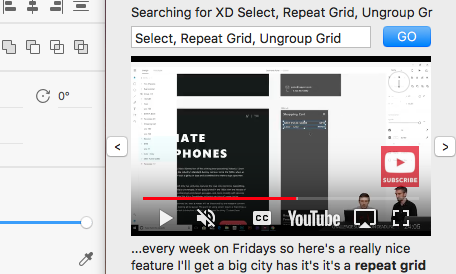
\includegraphics[width=\textwidth]{replay/figures/replay-old.png}
  \caption{Study 1 used this initial version of RePlay, shown here next to Adobe \textsc{xd}. It did not show video titles or timeline markers; instead it had arrow buttons next to each video to skip between that video's ranked clips. It also added the 3 most recent tools to the search query instead of one. }~\label{fig:replay-old}
%   \Description[A screenshot of an older version of RePlay.]{A screenshot of an older version of RePlay. Above the search field, the status area reads ``Searching for XD Select, Repeat Grid, Ungroup Grid''. Inside the search field it reads ``Select, Repeat Grid, Ungroup Grid''. It displays a video result with no title and a short caption excerpt underneath that includes the words ``repeat grid'' bolded.}
\vspace{-0.25in}
\end{figure}

\subsubsection{Contextual clip search was most useful for specific tasks}
Four participants said they tended to use RePlay when stuck trying to figure out how to do something specific. Three also said they used it to find out what a particular tool could do or how to use it. All but one participant worked on targeted tasks (see \autoref{table:study1_usage}). \textit{P3} wanted general resources for getting started with Sketch, and did not find RePlay helpful.

Three users recounted similar stories of searching for a particular question and quickly finding a clip within a video that answered it. \textit{P1} described searching for ``Make Symbol'' after clicking on the ``Make Symbol'' tool in Adobe \textsc{xd}. The answer he needed came from an auto-selected moment near the end of a 3-hour video. \textit{P1} added, \textit{``if I had searched for that myself I would've given up.''} Similarly, \textit{P5} found what he needed in a 1.5 hour video that was cued to a moment 20 minutes in. He was trying to create margins, and searched for ``layout grid'', and \textit{``The first video in the list showed me exactly what I needed to do''}, which was to check a box he hadn't noticed. \textit{P4} found RePlay useful for indicating that her specific goal was \textit{not} possible: she wanted to customize a grid system in Sketch and searched for ``grid settings'', but the caption excerpts indicated that none of the results mentioned customizing grids.

Contextual video clips sometimes invited opportunistic learning: \textit{P1} and \textit{P7} recounted instances where a video they were watching taught them something they didn't know and hadn't thought to look for. \textit{P1} continued watching the ``make symbols'' video as it described grouping and layering symbols. This part \textit{``wasn't originally what I was searching for but it was exactly what I needed ... [I] gained a lot more knowledge.''} \textit{P7} described how he \textit{``searched for `character styles' and actually found new information that I've never seen before''} about the Libraries panel.

\begin{figure*}[t!]
\centering
  \vspace{-0.2in}
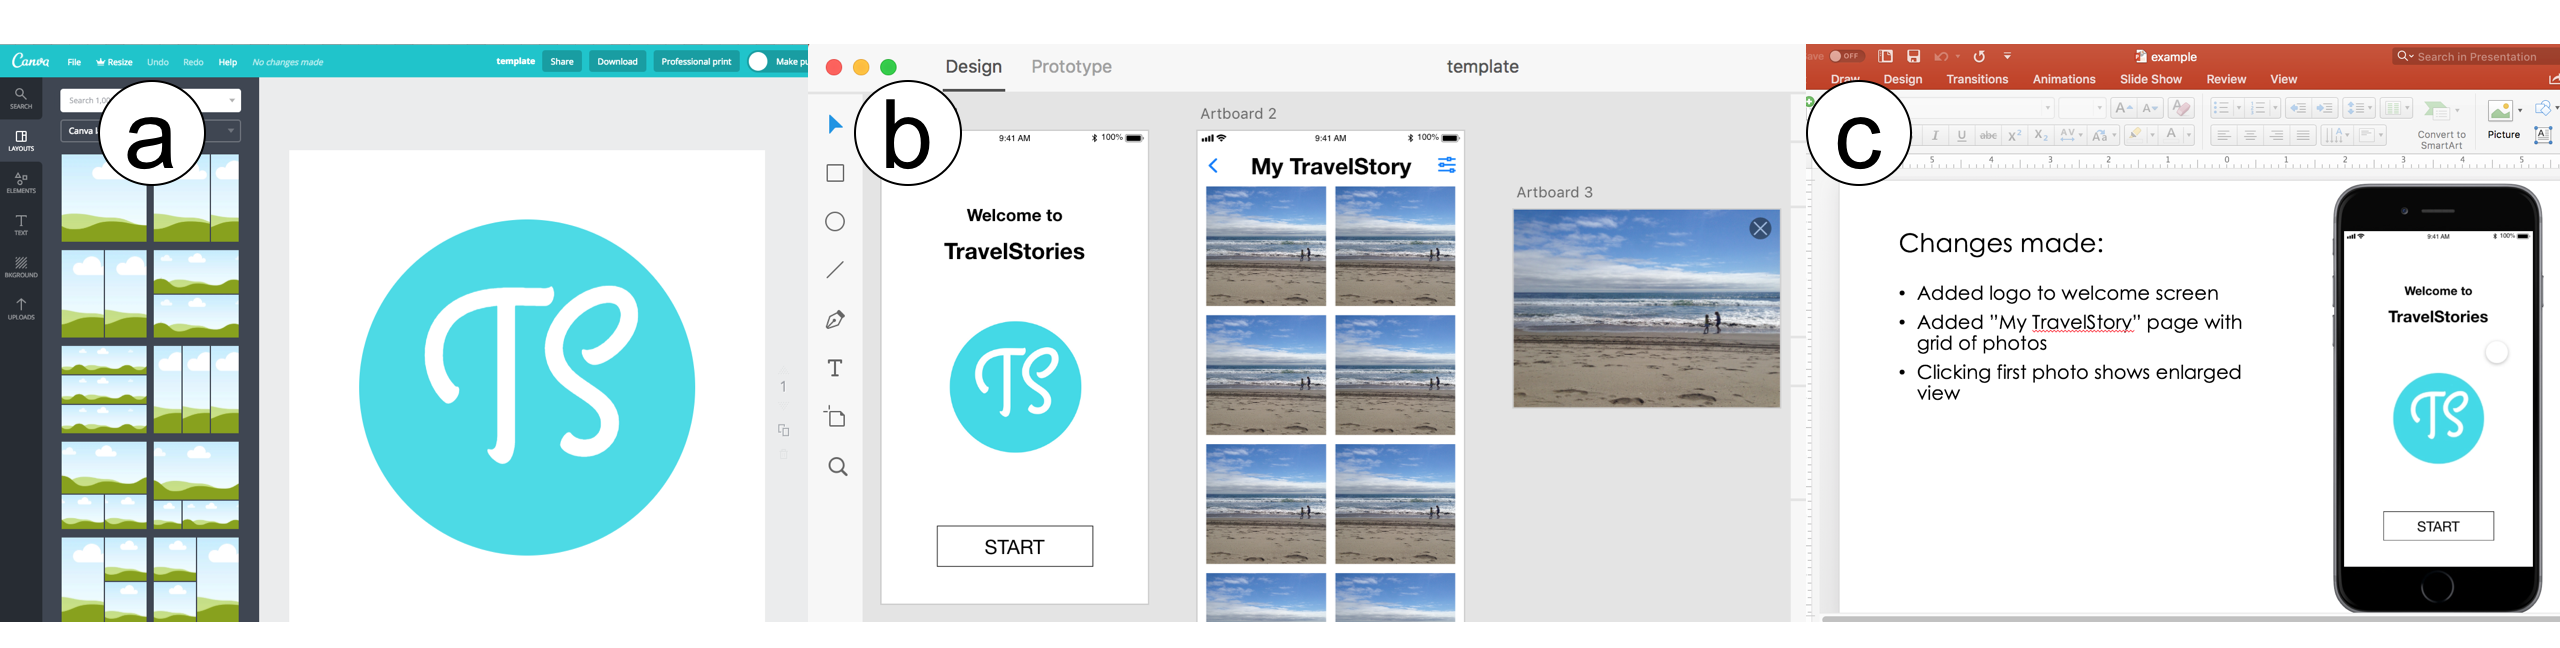
\includegraphics[width=\textwidth]{replay/figures/study2_task.png}
\vspace{-0.3in}
  \caption{Study 2 asked participants to make changes to an initial logo in Canva (a), update a prototype in Adobe \textsc{xd} (b), and make a presentation showing their changes in PowerPoint (c).}~\label{fig:replay-study2-task}
  \vspace{-0.2in}
%   \Description[Screenshots of the three template files participants were given.]{Screenshots of the three template files participants were given. The first is a blue circle with ``TS'' in the middle, shown in the Canva interface. The second is a wireframe design in Adobe XD with three phone screens, one that says ``Welcome to TravelStories'' with a Start button, one that says ``My TravelStory'' with a grid of photos below it, and one showing a photo at full size. The third is slide in PowerPoint with a screenshot of the wireframe on the right, and some text on the right that lists changes made to the design.}

\end{figure*}

%\vspace{0.1in}
\subsubsection{Tool context helps, but not in the search query}
All participants who searched with RePlay preferred deleting tool names from the query and instead typing their own. Five participants mentioned that including three tools in the query was too many, as it made the query too general. \textit{P3} said this was because the automatic query seemed \textit{``stuck on the last thing I did, which might not be relevant to what I'm thinking now.''} Both \textit{P4} and \textit{P5} said tool \textit{names} were not as useful because they wanted to search for an \textit{action}, not its constituent tools (\textit{e.g.,} ``rotate object'' or ``export nested artboard''). Higher-level activity inference may provide more useful assistance.

Two participants said they liked that RePlay populated the query with tool names because \textit{``coming up with the right search terms is really hard and I don't know the names of the tools [...] so it's nice not to have to think of them''} (\textit{P4}). Even \textit{P6}, the expert, said \textit{``I know how to use everything but if you asked me the names of the tools, I have no idea}.'' Participants appreciated that RePlay added the application name to the query, as it allowed them to \textit{``spend more brain power on the details of [the query]'' (P2)}. 

\subsubsection{Participants frequently switched between applications}
RePlay logged every time users switched between \textit{any} applications when it was running. Excluding system applications (such as Dock, Finder, and System Preferences), participants used an average of 17 different applications while RePlay was running ($SD\!=\!8$), and switched between applications a mean of every 6.6 minutes ($SD\!=\!8.5$min). If we exclude all continuous periods of over 3 hours (assuming that these sessions were breaks of some sort), this average lowers to every 2.5 minutes ($SD\!=\!1.8$min). This diverse app usage supports our motivation for supporting cross-app workflows.

\subsubsection{Improvements to RePlay}
Because participants thought that auto-including three tools was too many, Replay now includes only the most recent one. Four participants also mentioned that more general information like video titles would be helpful, as caption excerpts often seemed \textit{``out of context''} or \textit{``snatched out of middle of a sentence''} (\textit{P2}). Consequently, RePlay now includes video titles. Four participants wished they could watch videos at a larger size; RePlay now includes a resizable video player window. Two participants also mentioned that some video results did not pertain to the current application; RePlay now excludes results that do not mention the current application in the metadata or captions.

\section{Study 2: How does RePlay compare to current methods for video assistance?}

A between-subjects study ($n\!=\!24$) investigated how contextual assistance for multi-app activities might affect behavior compared to standard web video search. It found that contextual assistance can reduce time spent searching and navigating videos.

\subsection{Study procedure}
Participants were asked to imagine that they were designers working for a client developing a travel journal mobile app. To replicate a multi-app activity, the study task spanned three applications: Canva (\url{canva.com}), Adobe \textsc{xd}, and Microsoft PowerPoint. Participants were asked to improve and change an initial design for their client (\autoref{fig:replay-study2-task}). The task had both creative and technical requirements. Creative requirements included making the logo more travel-themed, adding visual appeal to the prototype welcome screen, and making a PowerPoint presentation to show to the client. Technical requirements included adding additional photos to a grid, rounding their corners, and recording a video walkthrough. If participants needed help, they were instructed to search for tutorial videos using either RePlay or YouTube in a web browser. RePlay participants were introduced to its features prior to the task. To ensure that all participants had access to the same resources, they were asked not to use other search engines or resources. Participants had 45 minutes to complete the task, and answered questions about their experience and help-seeking at the end. Participants were compensated with a \$15 gift card.

\subsubsection{Participants}
Twenty four participants (14 female) were recruited through online and paper advertisements on a university campus. Prior to the study, participants filled out a survey about their design experience. Participants were randomly assigned to either the RePlay ($n\!=\!12$) or Web ($n\!=\!12$) condition and counterbalanced based on experience. ``Novice'' was defined as completing at most two courses in design and reporting experience with at most two design applications. ``Experienced'' was defined as completing more than two courses in design or reporting experience with more than two design applications. Six of the 24 participants were ``experienced''. 

Participants rated their pre-study familiarity with each of the three study applications on a 5-point Likert Scale. Participants were generally familiar with Powerpoint ($mean\!=\!4.2$), and unfamiliar with Canva ($mean\!=\!1.5$) and Adobe \textsc{xd} ($mean\!=\!1.2$).
 
\subsubsection{Measures}
We were primarily interested in participants' search behavior. We measured the number of queries, their length, and time spent in the search interface. Qualitative measures included how participants determined which videos to watch and their navigation strategies (observed through screen recordings). We also gathered participant feedback in the RePlay condition on its features.

\subsection{Results}
RePlay participants averaged 3.3 queries each (33 total); Web participants averaged 3 queries each (24 total) ($x^2\!=\!1.42$, $df\!=\!1$, $p\!=\!.23$). Web participants typed longer queries ($mean\!=\!4.33$ words, $SD\!=\!1.41$) than RePlay participants ($mean\!=\!2.53$ words, $SD\!=\!0.59$)($t\!=\!2.52$, $df\!=\!15.98$, $p\!<\!.01$), because Web participants often manually added the application name, whereas RePlay auto-included it. 72\% of search queries were for Adobe \textsc{xd} and 28\% were for Canva; none were for PowerPoint since participants were more familiar with it. Four Web and two RePlay participants did not search for any assistance; we cover this in the Discussion.

Participants varied considerably in the amount of time and effort they spent. This is a challenge with a task that has both creative and technical components; people prioritize these components differently. Many participants spent a long time perfecting their design and had to be cut off after 45 minutes; others did the minimum required and finished in as few as 23 minutes. Because the task was open-ended, we did not compare completion times across participants. Our analysis focuses on search behavior. 

\begin{figure}[b!]
\centering
%\vspace{-0.25in}
  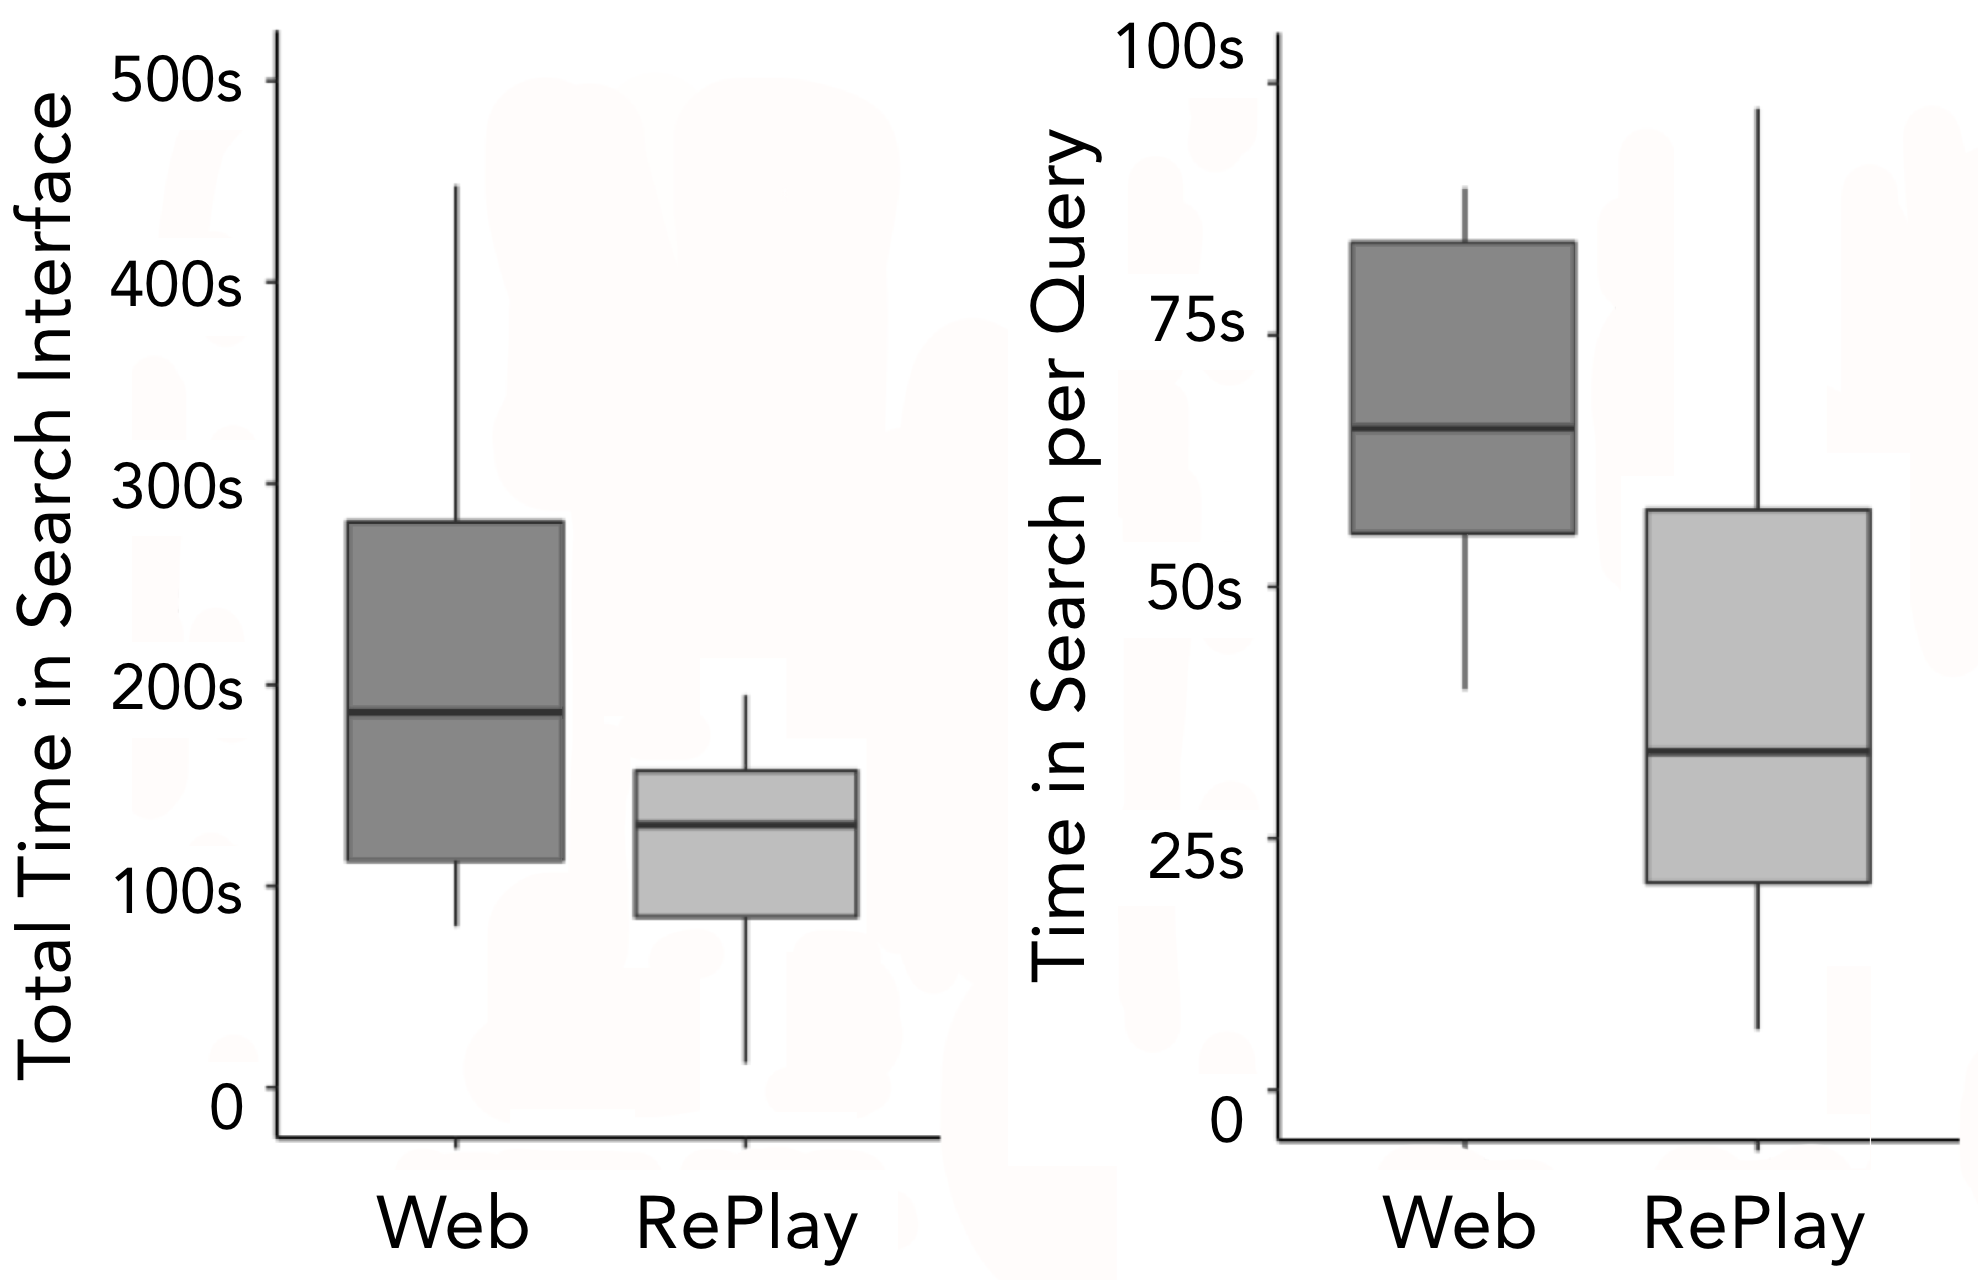
\includegraphics[width=1\textwidth]{replay/figures/study2_graphs.png}
  \caption{RePlay participants spent marginally less time overall in the search interface than Web participants ($p\!=\!.07$, left) and significantly less time \textit{per query} ($p\!=\!.02$, right).}~\label{fig:replay-study2-graphs}
  \vspace{-0.2in}
%   \Description[Two graphs showing the difference between RePlay and Web participants in time spent in the search interface.]{Two box plots showing the difference between RePlay and Web participants in time spent in the search interface. On the left, RePlay's box is slightly lower than Web's for total time in search (seconds). On the right, RePlay's box is significantly lower than Web's for time in search by query per person (seconds).}
\end{figure}

% Keep this somewhere? As a result, traditional completion time or completion rate are not suitable metrics. 

\subsubsection{Contextual assistance lessens time away from task}
Web participants spent nearly twice as long in the search interface ($mean\!=\!214.5$ seconds, $SD\!=\!127.1$) as RePlay ones ($mean\!=\!116.2$ seconds, $SD\!=\!58.9$). Due to the high variance and small sample size, the difference was marginally significant ($t\!=\!2.02$, $df\!=\!9.4$, $p\!=\!.07$) (\autoref{fig:replay-study2-graphs} left). When the time each participant spent in search is averaged by the number of queries they made, the difference is significant: RePlay participants spent about 40\% less time in search per query ($mean\!=\!42.83$ seconds, $SD\!=\!29.5$) than Web participants ($mean\!=\!72.62$ seconds, $SD\!=\!22.4$)($t\!=\!2.52$, $df\!=\!15.28$, $p\!=\!.02$) (\autoref{fig:replay-study2-graphs} right). Though RePlay pre-cached many video captions beforehand, we could not predict all queries users would make. Thus, some query responses in RePlay took up to two minutes. Because this latency could be reduced, we subtracted loading times in both conditions from the total time in search.

Easier navigation both within and between video results may explain why RePlay participants spent less time in the search interface per query. Web participants used various strategies for navigating within videos, including keyboard shortcuts to fast-forward and rewind, increasing video speed, and hovering over the timeline. Navigating between different video results in YouTube required selecting a video, watching or skipping through it to determine whether it was relevant, and if not, going back to the results page and selecting another. RePlay's timeline markers replaced many of these strategies, increasing efficiency: participants could first examine the timeline markers before deciding if and at what point to watch a video result. Eight RePlay participants hovered over timeline markers to read the caption previews, often hovering over multiple points before deciding where to watch. RePlay's panel interface also enabled participants to simultaeously play one video and examine others. We observed three participants do this, likely to decide whether another video was better without giving up on their first choice. One such participant said they wished for better visual cues of video relevance to help decide which to watch. Other participants browsed videos one at a time, perhaps to focus on the playing video.

% \begin{figure}[b!]
% \vspace{-0.25in}
% \centering
%   \includegraphics[width=0.9\textwidth]{replay/figures/study2_avgsearch.png}
%   \caption{Web participants spent significantly longer in the search interface \textit{per search query} than RePlay participants ($p=.02$). }~\label{fig:replay-study2-avgsearch}
% \end{figure}

\subsubsection{Search queries were action-oriented, not tool-oriented}
As in Study 1, participants removed tool names from queries. No participants in either condition used tool names. Instead, participants wrote action-oriented queries: the most common were ``crop photos'', ``round corners'', and ``record video.'' Despite RePlay adding the current tool name to the search field, in all instances but one, participants deleted the tool name from their query.

\begin{table}[t]
%\vspace{-0.35in}
\begin{tabular}{lllll}
\textit{RePlay Feature} & Title                   & Thumbnail               & Caption                 & Timeline                \\ 
\textit{Helpfulness}    & \multicolumn{1}{c}{2.8} & \multicolumn{1}{c}{3.1} & \multicolumn{1}{c}{2.5} & \multicolumn{1}{c}{4.2}
\end{tabular}
\caption{Average helpfulness ratings for RePlay's contextual features ($n\!=\!12$). Most participants found the timeline markers most helpful for determining which videos to watch.}~\label{table:study2_replayfeatures}
\vspace{-0.3in}
\end{table}

\subsubsection{Intra-video context is most helpful}
In interviews, participants rated timeline markers as the most helpful (4.2/5) (\autoref{table:study2_replayfeatures}). RePlay participants hovered over timeline markers a total of 69 times and clicked on markers 22 times. One participant mentioned that timeline markers provide a \textit{``scaffold of what to look for and where to start watching.''} Participants rated caption excerpt and video title as less helpful. A few participants mentioned ignoring titles and excerpts in favor of timeline markers and video thumbnails. Twice in each condition, participants selected the first video result even though the title mentioned the wrong application (Photoshop or Illustrator). This suggests that the video region is a strong magnet for people's attention.


%Tasks that require a context switch are perceived to take longer than tasks that don't. 
%Intra-person effect size for search interfaces is smaller than inter-person differences. To see the impact of search interfaces, need large n.
% One motivation for having the app do searching for you is that people aren't good at it. 

% Another participant found the timeline markers helped them \textit{extrapolate form the video where I should search for the content that I'm looking for. And it that one doesn't have it, I can just skip through and see other [points].''} general, participants found this feature helpful (4.11 rating on 5-point Likert scale). 
\section{Discussion \& Future Work}
Observations and feedback from the two studies suggest several opportunities for future work. 

\subsection{How Can Contextual Assistance aid Exploration?}
% assistance should not discourage exploration, but intervene when it is needed
% people explore because incremental cognitive load of exploration is small
% search is a one-time switch cost. if we can make the switching cost lower (by embedding in app and adding context) this should increase usage, and leaves people with more registers to focus on what they want to do.

Study 2 participants often preferred manually exploring when it would have been more efficient to search for help. The study's subjective, open-ended task may have encouraged such exploration. Only one participant used the best method to update the photo grid - using Adobe \textsc{xd}'s repeat grid feature to update all photos simultaneously - after learning about it in a video. Other participants used various less-efficient methods (\textit{e.g.}, un-grouping the repeat grid and manually adding and re-sizing photos). Because these methods achieved their desired goal, participants may not have thought to investigate whether a faster option existed.

Interface exploration and browser search each have shortcomings. Exploration is a common problem-solving strategy because it can be enjoyable, it builds on domain knowledge, and each individual action is low cost \cite{Lafreniere2014a, Rieman1996}. However, for novices especially, exploration is cumulatively slow, its learned knowledge is hard to integrate, and it induces a high cognitive load \cite{Tuovinen1999, Lafreniere2014a}. A limitation of learning unfamiliar domains via exploration is that people may settle for sub-optimal methods or strategies because they are unaware of a better alternative. Moving from an application to a web search can yield better results, but has a higher initial cost as it lurches people out of their task. We believe that contextual search has the potential to offer the benefits of both approaches without either of the drawbacks. 

Six participants in Study 2 did not search at all; most felt they could figure things out via exploration. One participant said they \textit{``felt like I could find it if I searched for it [in the interface], which I did. I was able to figure it out.''} Two other participants mentioned that they felt searching for help would be more time-consuming than trial-and-error exploration. One stated that he wanted to search for help, but \textit{``I knew I didn't have time. I wanted to complete the task so I just hacked it.''} If Study 2's result that contextual search reduces search time holds, these perceptions may change over time. RePlay's occasionally-slow loading times may have also affected this perception; prior work shows that a difference in latency of search results as small as 300ms can discourage people from searching \cite{Brutlag2009}.

How might contextual assistance encourage productive exploration while providing intervention when needed? While proactive support can be beneficial, a challenge is providing assistance without being too disruptive \cite{Matejka2011}. To minimize distractions, the RePlay interface mostly changes only in direct response to user input. However, novices may not even realize they need help, making proactive suggestions more valuable. For example, RePlay could automatically refresh video results when the user seems stuck, or suggest relevant queries when the user begins to search. Future work should examine how these alternatives might change people's behavior and workflows over time.
%will having assistance readily available change behavior over time? people have learned to guess their way to the solution and this is good in a lot of ways. but is there some interesting potential around a categorical strategy/behavior shift
% One Web participant said that he \textit{``almost always won't watch video because it's time-consuming...I usually prefer text-based help.''}. Similarly, another participant preferred text because \textit{``it's easier to parse rather than searching through a video.''} 

\subsection{What and How Much Context to Include?}
While logging recent tools can help suggest next steps \cite{Matejka2009}, we found that using recent tools explicitly in search queries is not useful. Participants in both studies did not use tool context in their queries, preferring action-oriented queries instead. Usage history is by definition retrospective (\textit{i.e.}, it describes what the user has already done). In contrast, search is often prospective (\textit{i.e.}, looking for something the user hasn't done yet). Tool context may only be helpful closer to where users interact with tools (\textit{e.g.,} as part of tooltips \cite{Grossman2010a}).
%can help divulge this information to users by increasing tools' information scent \cite{Pirolli2009}.

Interestingly, people used the same terms and concepts across different applications. Study 2 participants searched ``crop photos'' for both Canva and Adobe \textsc{xd} despite neither application having an explicit crop tool. This highlights both a challenge and an opportunity: people bring mental models that may not carry over into different applications. Study 1 suggested that displaying tool names may help people learn app-specific terminology. However, for both knowledge and speed reasons, users sometimes omit valuable terms. RePlay's interface benefits are reduced when users don't search using the same terms as videos. A natural language mapping \cite{Adar2014} between video captions (along with other natural language data like comments and tags) and the tools they mention may increase captions' value for search.

Finally, what other contextual information besides tool use might be helpful for identifying relevant videos? Liu \textit{et al.} \cite{Liu2020} showed that in addition to command logs, information about the use of layers and the time between interaction events can help segment usage logs from image editing tasks into subtasks. Similarly, information such as the name of the user's active layer might be helpful as additional context for a search query. Liu \textit{et al.} also found that the visual change and location of the user's edits were less useful for segmentation, but perhaps the visual content of the user's canvas or document could be used to identify videos with similar content. Future work should explore how we might collect and use such types of contextual information to search for help in an application-general way.

\subsection{What Design Challenges Remain?}
Many design decisions were motivated by our focus on cross-application workflows; \textit{e.g.,} showing results in a separate window in a consistent location. Showing all results together made it easy to browse multiple resources at once. However, some participants still preferred focusing on one video at a time. Future work should consider how different layouts influence browsing behaviors and which behaviors lead to more effective workflows.

Currently, users must explicitly whitelist an application for RePlay to capture its events. While this approach offers more privacy, it also adds burden for users.  Blacklisting, on the other hand, would allow RePlay to respond to all applications except for explicitly-omitted potentially-sensitive ones (\textit{e.g.,} Messages), offering broader benefits. For our initial studies, we chose the greater privacy of a whitelist. For real use, users could choose whitelist or blacklist, and/or RePlay could request approval for each new application, similar to websites that ask for a user's location.

\subsection{What Other Domains Might Benefit?}
RePlay's main insight is that given a source of user context, we can search, curate, and index into resources from a large corpus. RePlay demonstrates this approach using video; different activities (\textit{e.g.,} programming) may benefit from other types of content (\textit{e.g.,} text resources). RePlay could naturally be extended to any textual resource (or resource with textual metadata). Text results could be displayed as short summaries with clickable keywords to expand more detail~\cite{Ekstrand2011}. For detecting context, RePlay used Mac\-OS's accessibility \textsc{api}; other \textsc{os}s (\textit{e.g.} Windows \cite{Matejka2013}) also have similar \textsc{api}s. %Minor differences should not significantly affect RePlay's approach, as the user's query is still the primary search input.
Beyond software, RePlay's approach could extend to any domain for which online videos are abundant (\textit{e.g.,} physical building tasks). To detect activity context, one could augment physical tools with sensors \cite{Schoop2016, Lukowicz2004} or track body poses with wearable sensors or computer vision. A challenge for future work is to convert sensor or vision data into text searches, or to index videos using the sensor or vision data directly. 

% We used the application name, but the domain of the user's task may also be important for narrowing down results regarding multi-functional applications like Photoshop or Powerpoint.

% first study had a lot of retrospective context, was not helpful
% usage histor/state is retrospective and not always helpful for prospective search -- how address this without being clippy?
% eric horovitz
% how move forward with this and not end up with clippy? how to have good mixed initiative support?
% proactive variations: generate alternatives automatically and show them to you i already did it
% what about proactively suggesting search queries instead of videos/resources?

%All three participants in our field study almost exclusively typed their own search queries rather than using the ones RePlay provided. Using multiple recent tools explicitly in a search query takes the focus away from the specific question or tool the user wants help with. An alternative approach (suggested by \textit{P1}) could instead show recent tools as clickable elements for quick searches, while also providing a search box for user-generated queries.

% Future work: use prefab methods to get visual stuff too, could search with that

% \subsection{The First Result is Most Relevant for Context}
% Effective search interfaces should not only present relevant results, but also present the most relevant results at the top of the set [Hearst]. As we observed in Study 2, people tend to habitually choose the first result provided, expecting it to contain the most relevant information needed.

\section{Conclusion}
This paper introduced an application-independent approach for contextually presenting videos and a demonstration of this approach in the RePlay system. RePlay shows how system accessibility features and video captions can be used to detect context and search within videos in a flexible, domain-general way. Like curb cuts or closed captioning \cite{Rose2002}, RePlay demonstrates how accessibility features can provide universally-beneficial assistance. 
Expanding accessibility and increasing cross-app consistency through guidelines and enforcement would benefit everyone. It would also expand application tailoring, integration, and assistance with systems like RePlay. Two studies demonstrated that cross-app contextual video assistance helps users spend more time on their task and less time searching for help. We also observed how contextual assistance can sometimes be at odds with peoples' desire to explore and tinker, and that the context most easily accrued from software usage may not always be the most relevant. Future work should investigate these challenges and examine how contextual help affects workflows in the real world through a longitudinal study. This work brings us one step closer to leveraging the wisdom of the Web for personalized, just-in-time learning.

\section{Acknowledgments}
We are thankful to Michelle Lee for her assistance in conducting Study 2, and to all study participants for their time and feedback. This work was supported in part by NSERC and Adobe Research.
